\section{Sentiments and Clusters}
We train a deep convolutional network on the Sentibank \cite{sentibank} dataset, to classify images in a set of 2079 Adjective noun pairs, each of which have been assigned sentiments using crowd sourced effort. This network gave a top 5 match accuracy for the test dataset of 75\%. 
\par
The trained visual sentiment detector was then used on chronologically sampled frames from the vine videos collected. We sample 1 image per second for the 7 second long clips and hence now each video was being represented as a vector of 7 sentiment transition values. The main aim of this was to see if users are trying to tell stories in these short vine videos. One of the evidences of this would be clustering of similarly transitioning visual sentiments for videos across the dataset. 

\begin{figure}
\centering
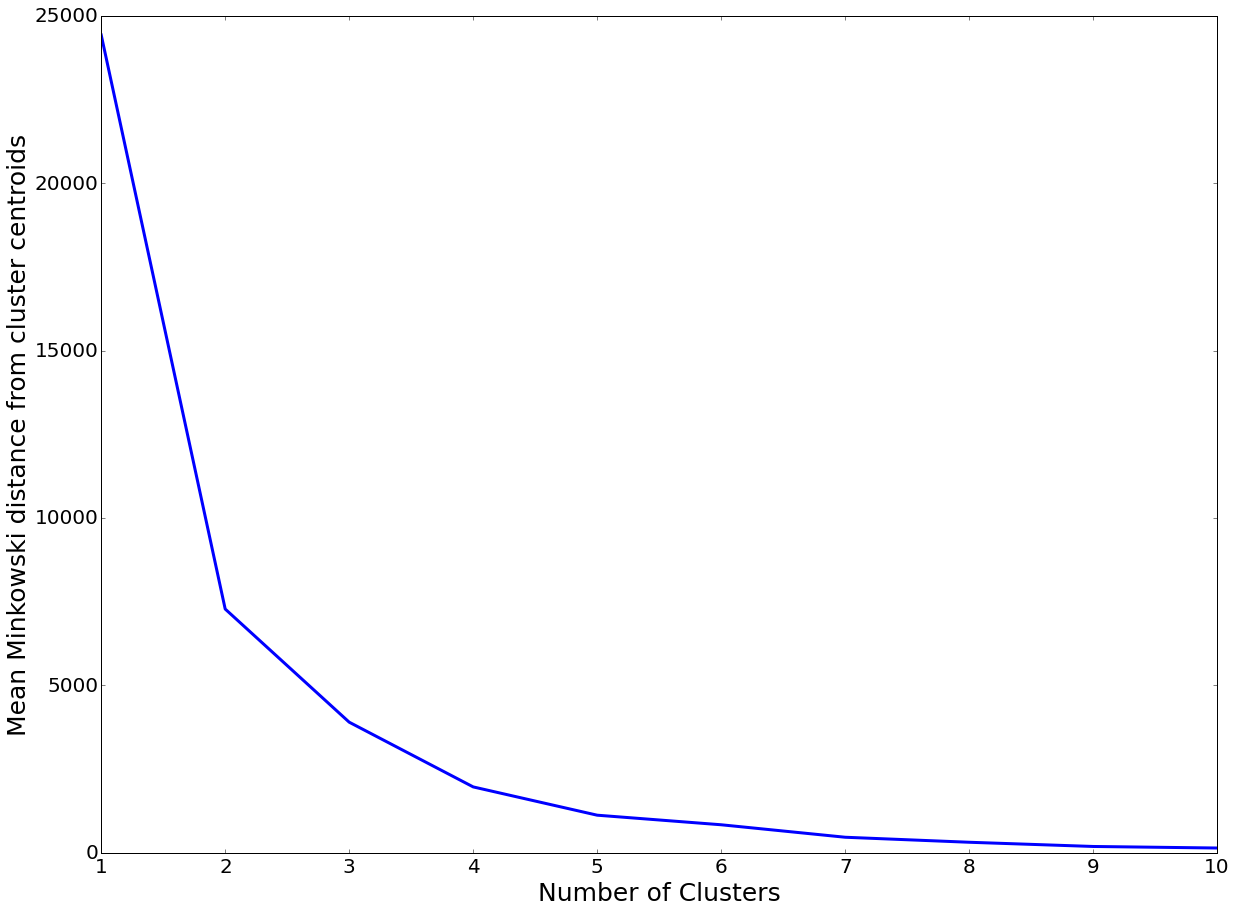
\includegraphics[width=\columnwidth]{plots/grouping_graph_clusters}
\caption{\textsl{This graph shows the variation of average minkowski distance of a sentiment vector from a cluster centroid for a given choice of K. The k is varied from 1 to 10.}}
\label{fig:elbow_points}
\end{figure}

\begin{figure}
\centering
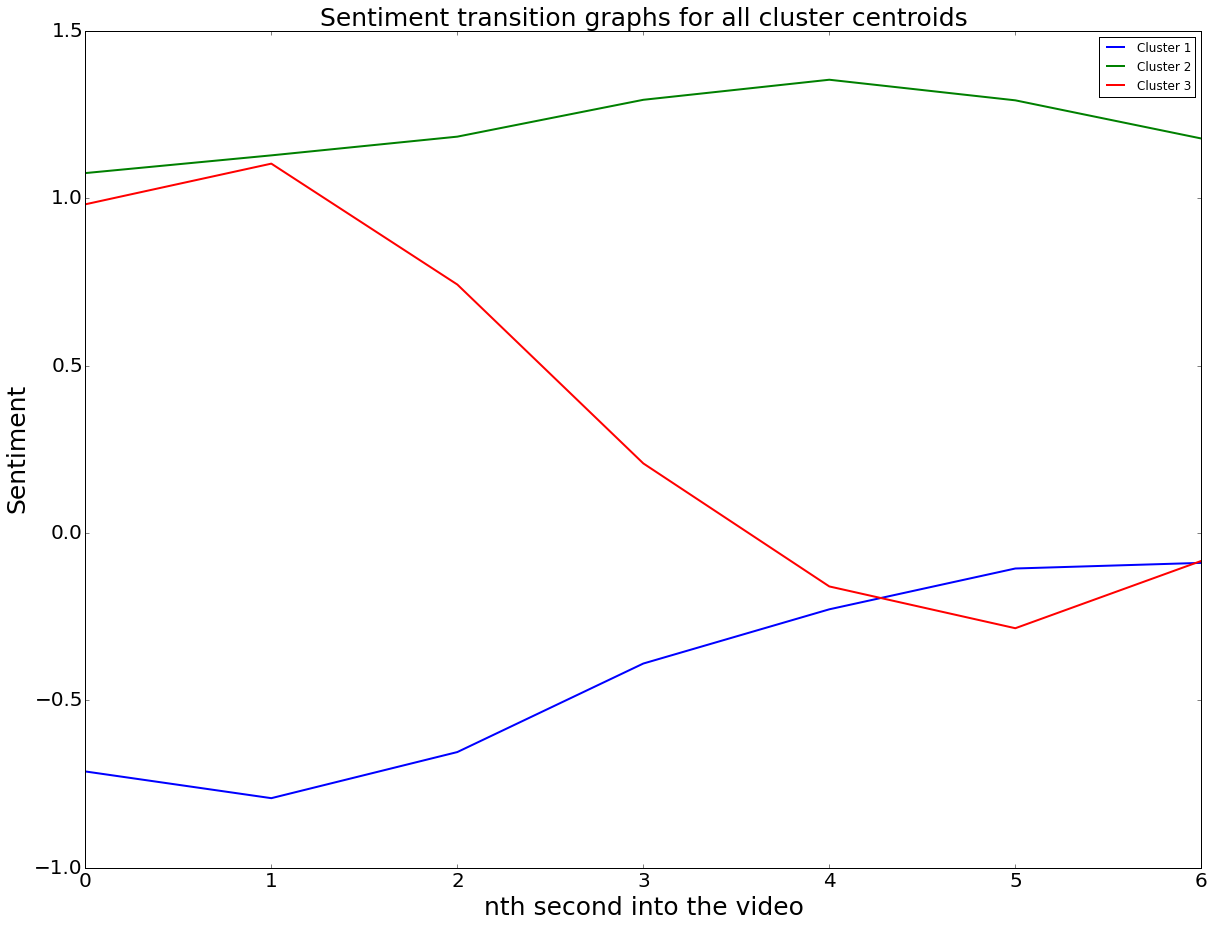
\includegraphics[width=\columnwidth]{plots/3_clusters_transitions}
\caption{\textsl{Sentiment values transitions for the centroids the clusters when K = 3.}}
\label{fig:3_clusters}
\end{figure}

\begin{figure}
\centering
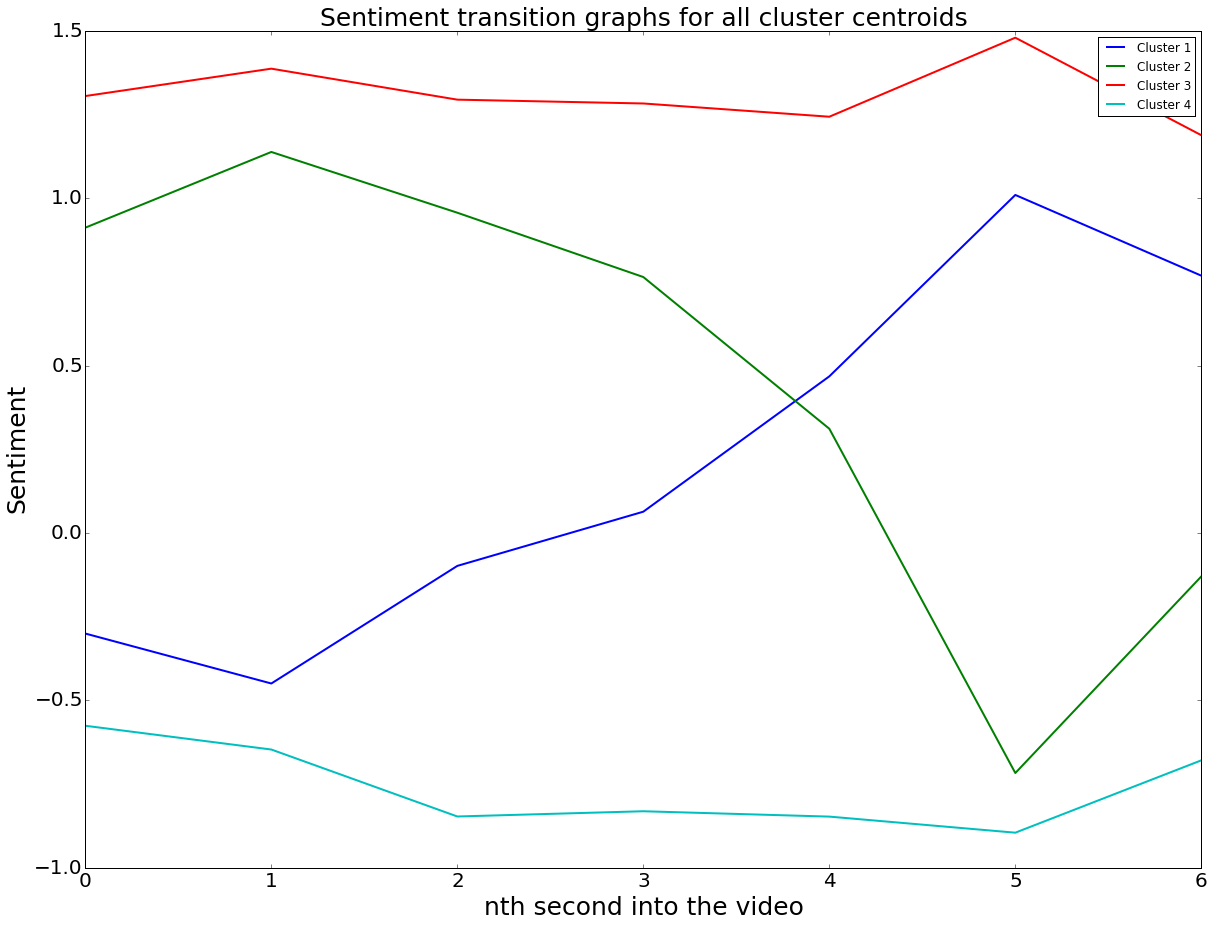
\includegraphics[width=\columnwidth]{plots/4_clusters_transitions}
\caption{\textsl{Sentiment values transitions for the centroids the clusters when K = 4.}}
\label{fig:4_clusters}
\end{figure}

\begin{figure}
\centering
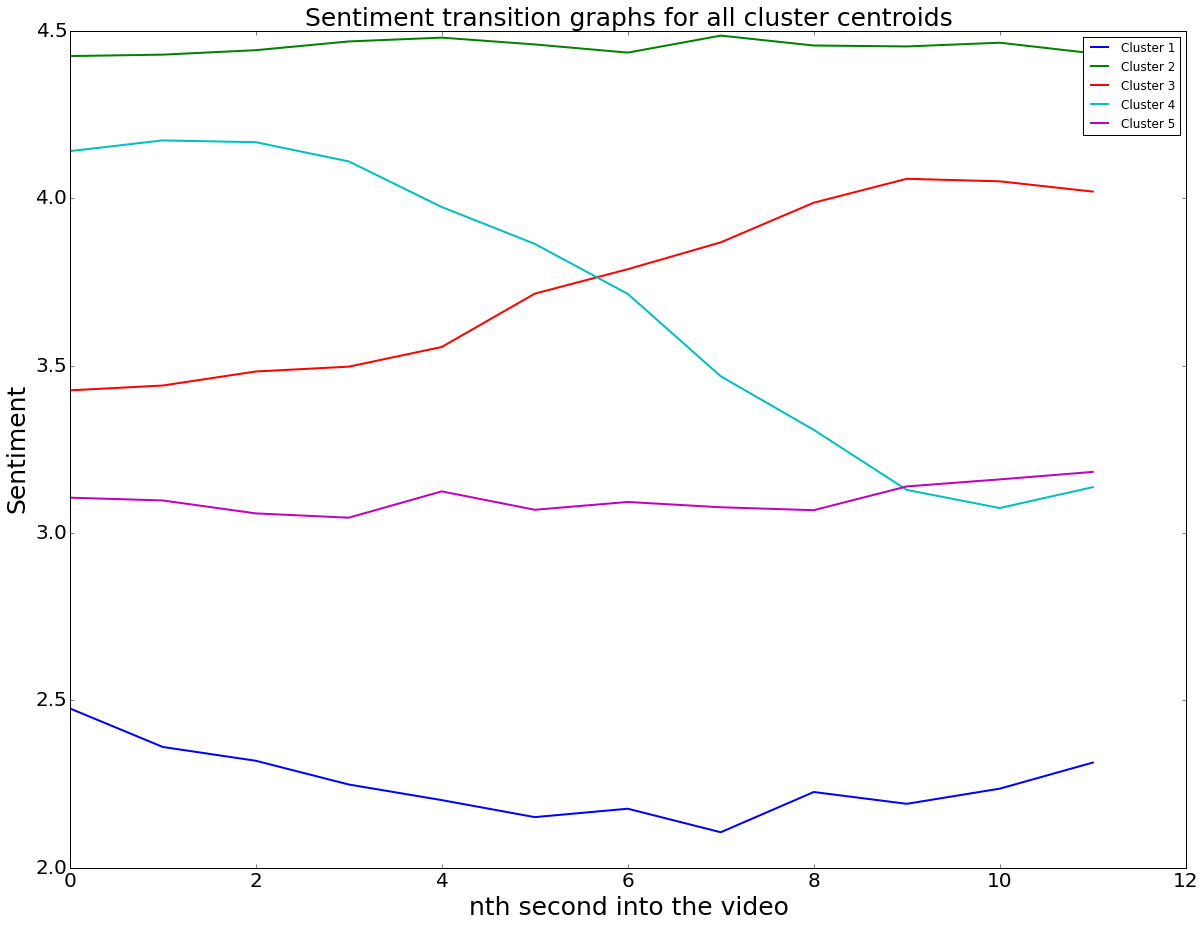
\includegraphics[width=\columnwidth]{plots/5_clusters_transitions}
\caption{\textsl{Sentiment values transitions for the centroids the clusters when K = 5.}}
\label{fig:5_clusters}
\end{figure}